Under the assumption that the UTA provided drone for testing will operate in a particular frequency band for its rotor spin; The ArGoose system will be calibrated to identify this frequency to detect and identify directional components for the intruding drone. To accomplish this goal, the system will contain a continuous detecting loop utilizing a six-sided hexagonal sound array attached to a Raspbery Pi monitoring system. When the drone enters within the range of the system, the audio sensors will pick up the frequency assigned and forward this information to an internal audio to digital converter located within the Respeaker sensor array. After conversion, the data will be forwarded to a system called ODAS (Open Embedded Audition System) that will be loaded on the Raspberry Pi. This open-source software contains the foundation used to establish directional audio detection. With ODAS as a foundation, custom code will be constructed to limit the detection bandwidth to the necessary frequencies and eliminate “noise” that is detected and unimportant for our purpose. After proper processing and successful drone detection, the system will activate its secondary sensor suite, at this time an RF detection system and identify the RF signal of a nearby drone. The RF for drones follow the same pattern as the rotor sound generation and the detection algorithm will locate based on the particular bandwidth that a drone may operate in. By using the directionality provided by ODAS and the sound array, the RF will be focused on a particular area to detect the offending drone, so as to limit cross contamination from multiple sources. With verification of these two systems both detecting a possible drone, The data collected by ODAS to identify directionality as well as the RF details collected on the operating range of the drone and any telemetry that has been calculated will be forwarded to a web-based user interface for human assessment and action.
\begin{figure}[h!]
    \centering
    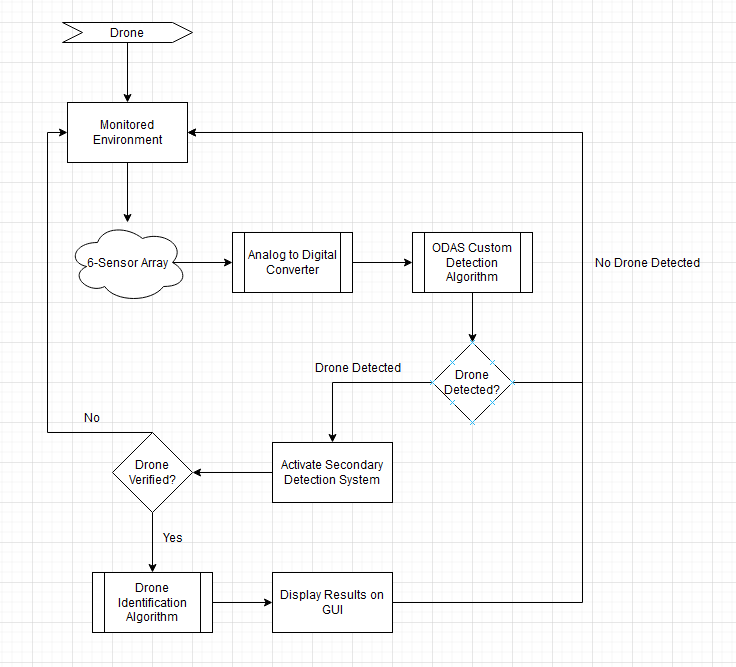
\includegraphics[width=1\textwidth]{images/argoose_schematic.png}
    \caption{Drone Detection Prototype Schematic}
\end{figure}